% This example uses the 'minted' package, so you need to run the compiler with 
% the '-shell-escape' option, i.e.
% 	pdflatex -shell-escape example.tex
% Additionally, you must have the 'pygmentize' program installed, which is part of 
% the 'Pygments' package (https://pygments.org/)
% !TEX option = -shell-escape
\documentclass[aspectratio=1610, english]{beamer} 
% Jeśli chcesz otrzymać prezentację w języku polskim, to, powyżej, zamień „english” na „polish”
\usepackage{babel}
\makeatletter
\@ifclasswith{beamer}{polish}{
	\usepackage{polski}
}
\makeatother
\usepackage[utf8]{inputenc}
\usepackage{listings} % We want to put listings
\usepackage{minted}   % We want to put listings
\usepackage{multirow}
\usepackage{amsmath}
\usepackage{physics}

\mode<beamer>{ 	% In the 'beamer' mode
	\definecolor{links}{HTML}{2A1B81}
	\hypersetup{
		pdfpagemode=FullScreen,                 % Enable Full screen mode
		colorlinks,
		linkcolor=,
		urlcolor=links
	}
	\usetheme[parttitle=rightfooter]{AGH}       % Show part title in right footer
	%\usetheme[nosidebar]{AGH}                  % Do not show sidebar on non-title slides
	%\usetheme[nosidebar, margins=1em]{AGH}     % Do not show sidebar on non-title slides and set both margins (left / right) to 1em
	%\usetheme[dark]{AGH}                       % Use dark background
	%\usetheme[dark, parttitle=leftfooter]{AGH} % Use dark background and show part title in left footer
}
\mode<handout>{	% In the 'handout' mode
	\hypersetup{pdfpagemode=None}		
	\usepackage{pgfpages}
	\pgfpagesuselayout{4 on 1}[a4paper,border shrink=5mm,landscape]	% Show 4 slides on 1 page
	\pgfpageslogicalpageoptions{1}{border code=\pgfusepath{stroke}}
	\pgfpageslogicalpageoptions{2}{border code=\pgfusepath{stroke}}
	\pgfpageslogicalpageoptions{3}{border code=\pgfusepath{stroke}}
	\pgfpageslogicalpageoptions{4}{border code=\pgfusepath{stroke}}
  	\usetheme{boxes}
  	\addheadbox{structure}{\quad\insertpart\hfill\insertsection\hfill\insertsubsection\qquad}          % Content of header
 	\addfootbox{structure}{\quad\insertshortauthor\hfill\insertframenumber\hfill\insertsubtitle\qquad} % Content of footer
}

\AtBeginPart{ % At begin part: display its name
	\frame{\partpage}
} 

%  ICCS TITLE PAGE
% \author[Sebastian Dziura]{Tomasz Rybotycki\inst{1,2,3} \and Sebastian Dziura\inst{1} \and Piotr Gawron\inst{1,2}%
% %   \\{\scriptsize \href{mailto:sdziura@agh.edu.pl}{sdziura@agh.edu.pl}}%
% }
% \date{}
% \title[AQML4MSC]{Auto Quantum Machine Learning for Multisource Classification}
% \institute[AGH]{
% 		\inst{1}Center of Excellence in Artificial Intelligence\newline
% 		AGH University, al. Mickiewicza 30, 30-059 Cracow, Poland
% 	\and
% 		\inst{2}Nicolaus Copernicus Astronomical Center\newline
% 		Polish Academy of Sciences, ul.Bartycka 18, 00-716 Warsaw, Poland
% 	\and
% 		\inst{3}Systems Research Institute\newline
% 		Polish Academy of Sciences, ul. Newelska 6, 01-447 Warsaw, Poland
% }

% AGH SEMINAR TITLE PAGE
\author[Sebastian Dziura]{\textbf{Sebastian Dziura}
   {\scriptsize \newline{Supervisor: \textbf{dr hab. inż. Piotr Gawron}} \newline {Auxilary supervisor: \textbf{dr inż. Tomasz Rybotycki}}}%
}
\date{}
\title[AQML4MSC]{Quantum machine learning algorithms for multi-source data classification}
\institute[AGH]{
		\inst{} Center of Excellence in Artificial Intelligence\newline
		AGH University, al. Mickiewicza 30, 30-059 Cracow, Poland
}


\logo{
    
\includegraphics[width=1cm]{fig/ceai-logo-icon.png} % Grafika widoczna ma każdym ze slajdów
}         

%%%%%%%%%%% Configuration of the listings package %%%%%%%%%%%%%%%%%%%%%%%%%%
% Source: https://en.wikibooks.org/wiki/LaTeX/Source_Code_Listings#Using_the_listings_package
%%%%%%%%%%%%%%%%%%%%%%%%%%%%%%%%%%%%%%%%%%%%%%%%%%%%%%%%%%%%%%%%%%%%%%%%%%%%
\lstset{ %
  backgroundcolor=\color{white},   % choose the background color
  basicstyle=\footnotesize,        % the size of the fonts that are used for the code
  breakatwhitespace=false,         % sets if automatic breaks should only happen at whitespace
  breaklines=true,                 % sets automatic line breaking
  captionpos=b,                    % sets the caption-position to bottom
  commentstyle=\color{green},      % comment style
  deletekeywords={...},            % if you want to delete keywords from the given language
  escapeinside={\%*}{*)},          % if you want to add LaTeX within your code
  extendedchars=true,              % lets you use non-ASCII characters; for 8-bits encodings only, does not work with UTF-8
  frame=single,	                   % adds a frame around the code
  keepspaces=true,                 % keeps spaces in text, useful for keeping indentation of code (possibly needs columns=flexible)
  keywordstyle=\color{blue},       % keyword style
  morekeywords={*,...},            % if you want to add more keywords to the set
  numbers=left,                    % where to put the line-numbers; possible values are (none, left, right)
  numbersep=5pt,                   % how far the line-numbers are from the code
  numberstyle=\tiny\color{gray},   % the style that is used for the line-numbers
  rulecolor=\color{black},         % if not set, the frame-color may be changed on line-breaks within not-black text (e.g. comments (green here))
  showspaces=false,                % show spaces everywhere adding particular underscores; it overrides 'showstringspaces'
  showstringspaces=false,          % underline spaces within strings only
  showtabs=false,                  % show tabs within strings adding particular underscores
  stepnumber=2,                    % the step between two line-numbers. If it's 1, each line will be numbered
  stringstyle=\color{cyan},        % string literal style
  tabsize=2,	                   % sets default tabsize to 2 spaces
  title=\lstname,                  % show the filename of files included with \lstinputlisting; also try caption instead of title
                                   % needed if you want to use UTF-8 Polish chars
}
%%%%%%%%%%% Configuration of the minted package %%%%%%%%%%%%%%%%%%%%%%%%%%
\setminted[C++]{frame=single,linenos}

%%%%%%%%%%%%%%%%%
\begin{document}
\maketitle


%%%%%%%%%%%%%%%%%%%%%%%%%%%%%%%%%%%%%%%%%%%%%%%%%%%%%%%%%%%%%%%%%%%%%%%%%%%%%%%%%%%%%%%%%%%%%%%%%%%%%%%%%%%%%%%%%%%%%%%%%%%%%%%%%%%%%%%%%%%%%%%%%%%%%%%%%%%%%%%%%%%%%%%%%%%%%%%%%%%%%%%%%%%%%%%%
%%%%%%%%%%%%%%%%%%%%%%%%%%%%%%%%%%%%%%%%%%%%%%%%%%%%%%%%%%%%%%%%%%%%%%%%%%%%%%%%%%%%%%%%%%%%%%%%%%%%%%%%%%%%%%%%%%%%%%%%%%%%%%%%%%%%%%%%%%%%%%%%%%%%%%%%%%%%%%%%%%%%%%%%%%%%%%%%%%%%%%%%%%%%%%%%
%%%%%%%%%%%%%%%%%%%%%%%%%%%%%%%%%%%%%%%%%%%%%%%%%%%%%%%%%%%%%%%%%%%%%%%%%%%%%%%%%%%%%%%%%%%%%%%%%%%%%%%%%%%%%%%%%%%%%%%%%%%%%%%%%%%%%%%%%%%%%%%%%%%%%%%%%%%%%%%%%%%%%%%%%%%%%%%%%%%%%%%%%%%%%%%%
% \part{Introduction}
\begin{frame}[t, fragile]{{Multisource}}
	\begin{block}<1->{Multisource data}
		Information about a single observed object collected from multiple complementary sources.
	\end{block}
	\setlength{\columnsep}{0pt}
	\begin{columns}[c,onlytextwidth]
		\column{0.5\textwidth}
		\vspace{3mm} \\
		Multisource dataset includes:
		\begin{itemize}[<+(1)-|alert@+(1)>]
			\item different data origin,
			\item multiple modalities,
			\item different timing.
		\end{itemize}
		\column{0.5\textwidth}
		\vspace{3mm} \\
		\includegraphics<2>[width=1.2\textwidth]{fig/ms_cameras.png}
		\includegraphics<3>[width=1.2\textwidth]{fig/ms_multimodal.png}
		\includegraphics<4>[width=1.2\textwidth]{fig/ms_change.png}
	\end{columns}
\end{frame}

\begin{frame}[t,fragile]{{Multisource Information Fusion (MSIF)}}
	\begin{block}<1->{Multisource Information Fusion (MSIF)}
		MSIF is a process to aggregate and transform multisource data into useful information to e.g.\
		obtain richer and more accurate decision outcomes
	\end{block}
	\setlength{\columnsep}{0pt}
	\begin{columns}[c,onlytextwidth]
		\column{0.4\textwidth}
		\vspace{1cm} \\
		We can distinguish three \textbf{levels of fusion}:
		\begin{itemize}[<+(1)-|alert@+(1)>]
			\item Data-level fusion
			\item Feature-level fusion
			\item Decision-level fusion
		\end{itemize}
		\column{0.6\textwidth}
		\vspace{1cm} \\
		\includegraphics<2>[width=1.2\textwidth]{fig/Data_Fusion-crop.pdf}
		\includegraphics<3>[width=1.2\textwidth]{fig/Feature_Fusion-crop.pdf}
		\includegraphics<4>[width=1.2\textwidth]{fig/Decision_Fusion-crop.pdf}
	\end{columns}
\end{frame}

\begin{frame}[fragile]{{Quantum Machine Learning (QML)}}
	\begin{figure}
		\centering
		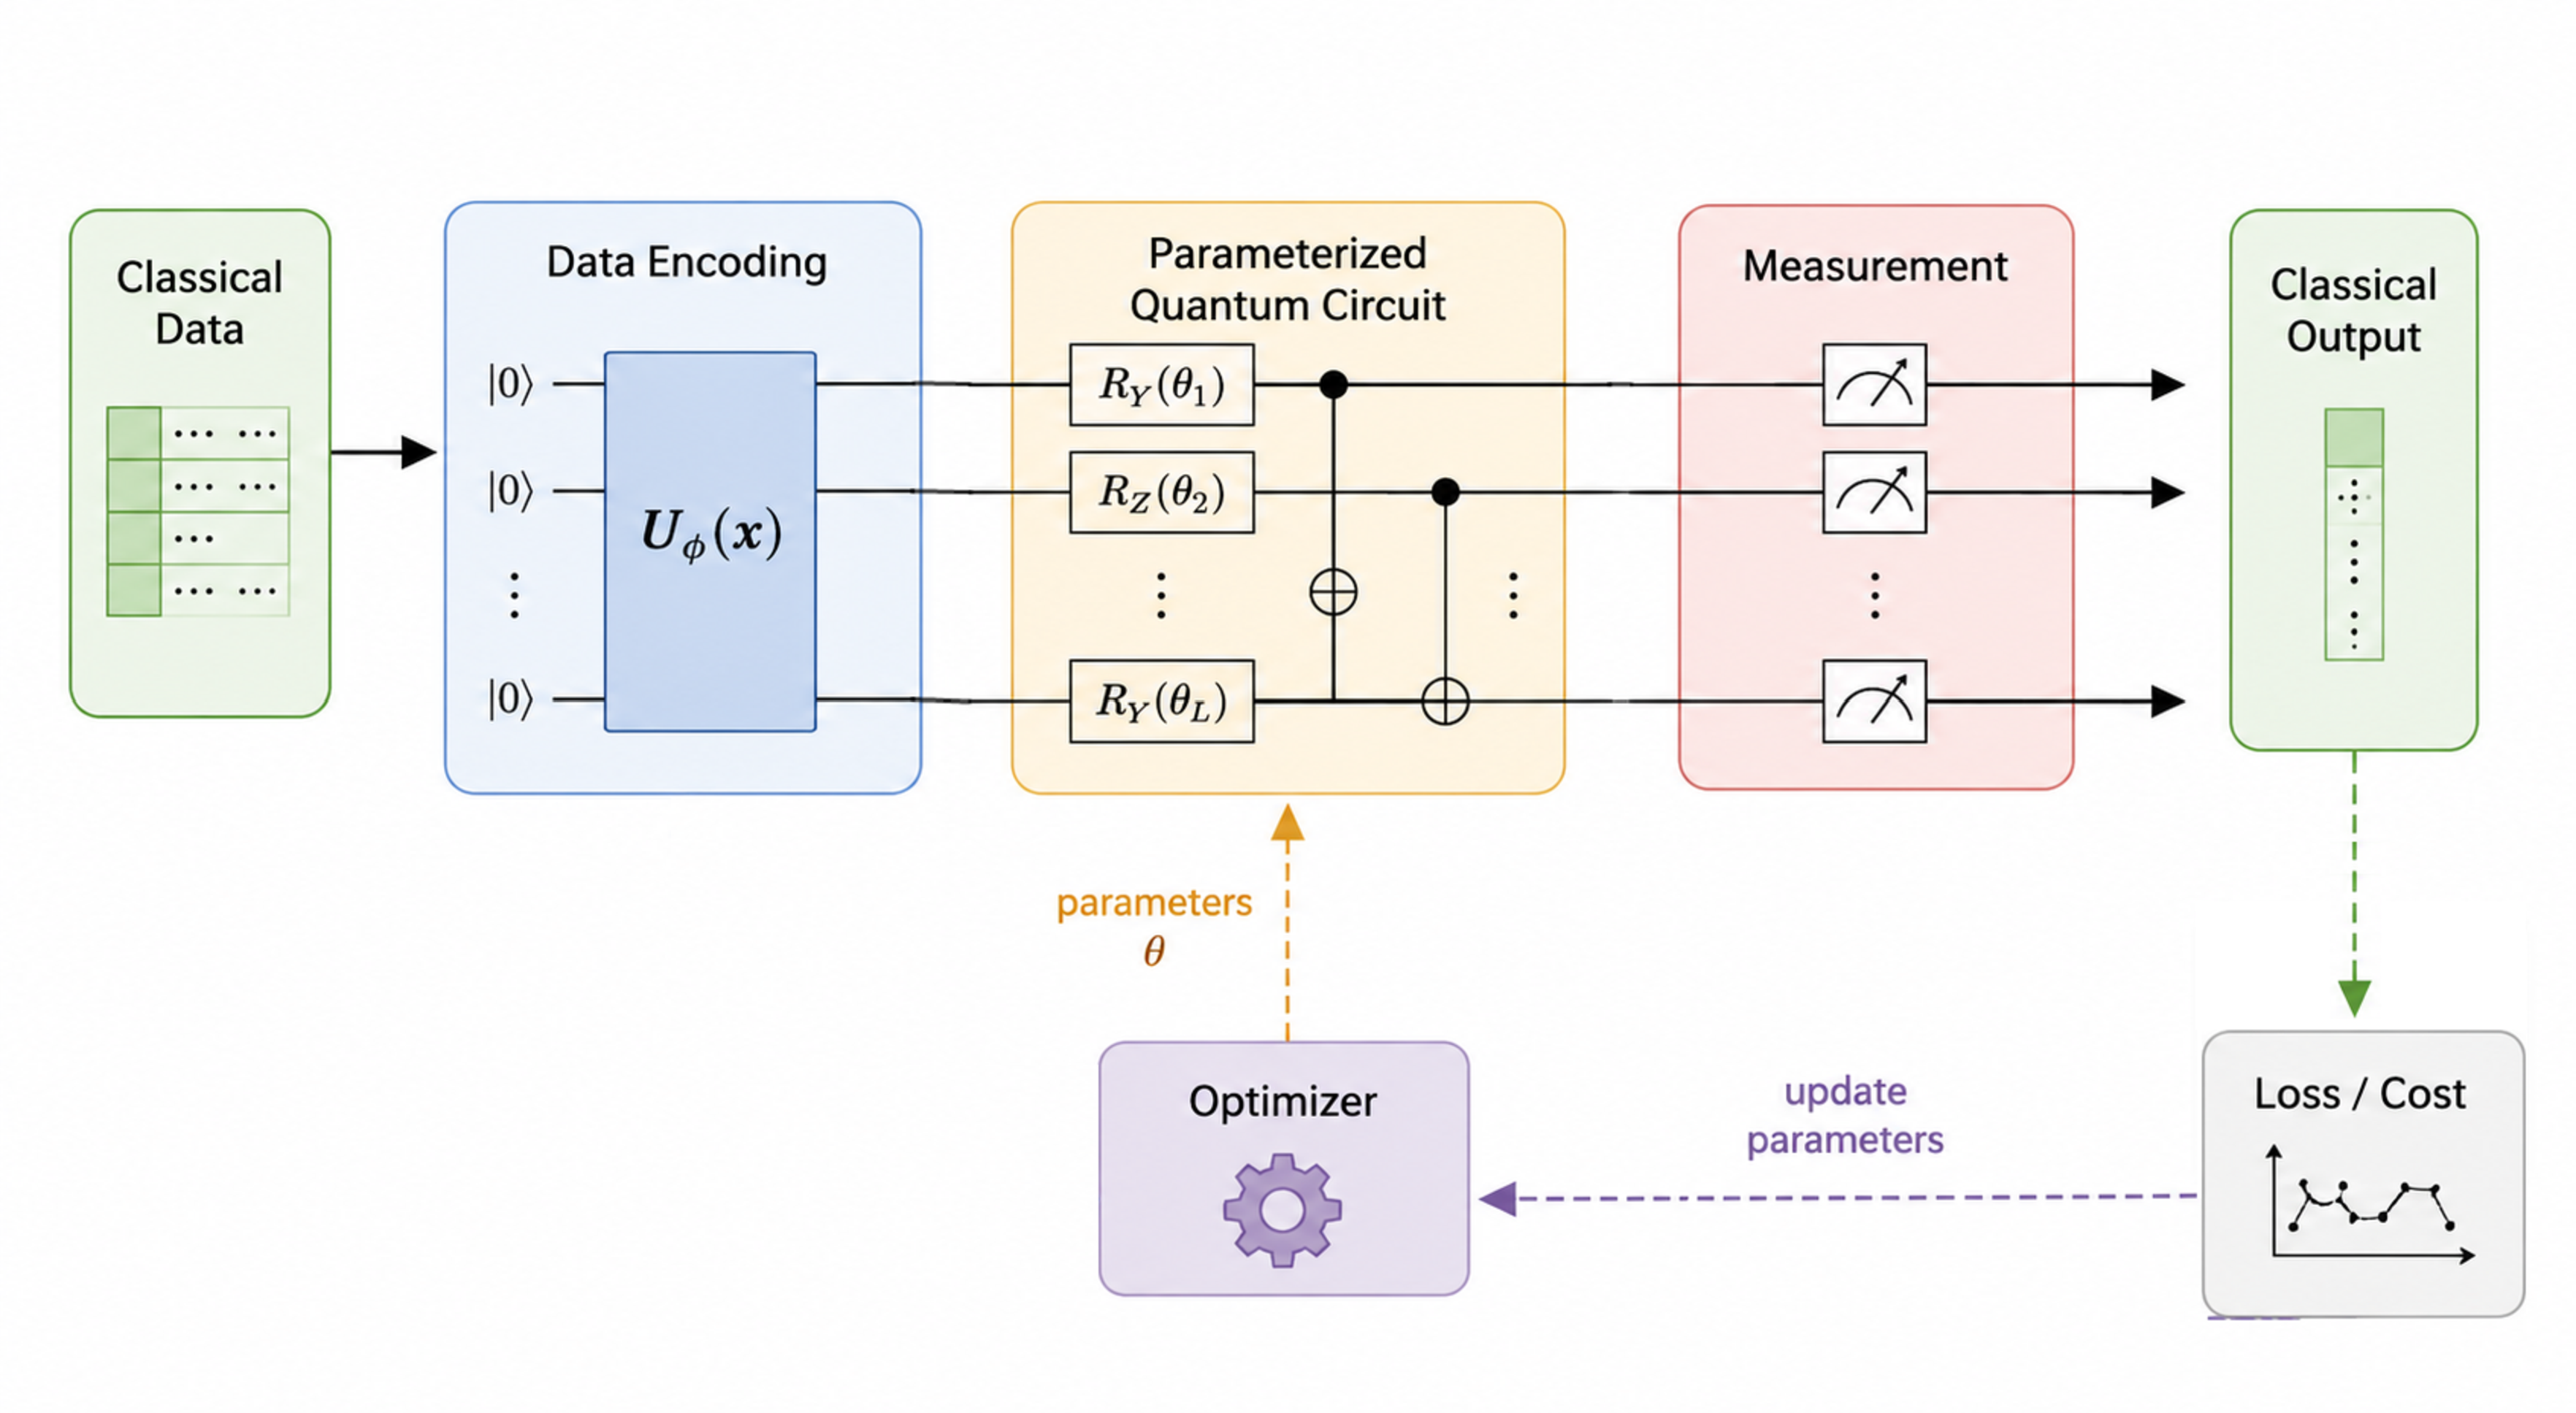
\includegraphics[width=1.0\textwidth]{fig/qml_2.pdf}
		\label{fig:qml}
	\end{figure}
\end{frame}

\begin{frame}[t,fragile]{{Quantum Embedding}}
	\begin{block}<1->{Quantum Embedding}
		A representation method where classical data is mapped into a quantum state or quantum feature space, enabling processing via quantum circuits
	\end{block}
	\setlength{\columnsep}{0pt}
	\begin{columns}[c,onlytextwidth]
		\column{0.4\textwidth}
		\vspace{1cm} \\
		Examples of quantum embedding methods:
		\begin{itemize}[<+(1)-|alert@+(1)>]
			\item Basis embedding
			\item Angle embedding
			\item Amplitude embedding
		\end{itemize}
		\column{0.6\textwidth}

		\only<2>{
			\begin{center}
				\fbox{$n$ bits = $n$ qubits}
			\end{center}
			\textbf{Classical data:}
			$$ \mathbf{x} = \begin{bmatrix} 1 & 0 & 1 \end{bmatrix} $$
			\textbf{Quantum state:}
			$$ \ket{\psi} = \ket{101} $$
		}
		\only<3>{
			\begin{center}
				\fbox{$n$ features = $n$ qubits}
			\end{center}
			\textbf{Classical data:}
			$$ \mathbf{x}  = \begin{bmatrix} \frac{\pi}{4} & \frac{\pi}{3} & \frac{\pi}{2} \end{bmatrix} $$
			\textbf{Quantum state:}
			$$ \ket{\psi} = R_x\left(\frac{\pi}{4}\right) \ket{0} \otimes R_x\left(\frac{\pi}{3}\right) \ket{0} \otimes R_x\left(\frac{\pi}{2}\right) \ket{0} $$
		}
		\only<4>{
			\begin{center}
				\fbox{$2^n$ features = $n$ qubits}
			\end{center}
			\textbf{Classical data:}
			$$ \mathbf{x} = \begin{bmatrix} \frac{1}{4} & \frac{1}{\sqrt{2}} & \frac{1}{2} & \frac{\sqrt{3}}{4} \end{bmatrix} $$
			\textbf{Quantum state:}
			$$ \ket{\psi} = \frac{1}{4}\ket{00}  + \frac{1}{\sqrt{2}}\ket{01}  + \frac{1}{2}\ket{10}  + \frac{\sqrt{3}}{4}\ket{11}  $$

		}
	\end{columns}
\end{frame}

\begin{frame}[fragile]{{Variational Layers}}
	\begin{tikzpicture}[remember picture, overlay]
		% Image 1: Top Left
		\node<3-> at ([shift={(3cm,-3cm)}]current page.north west)
		{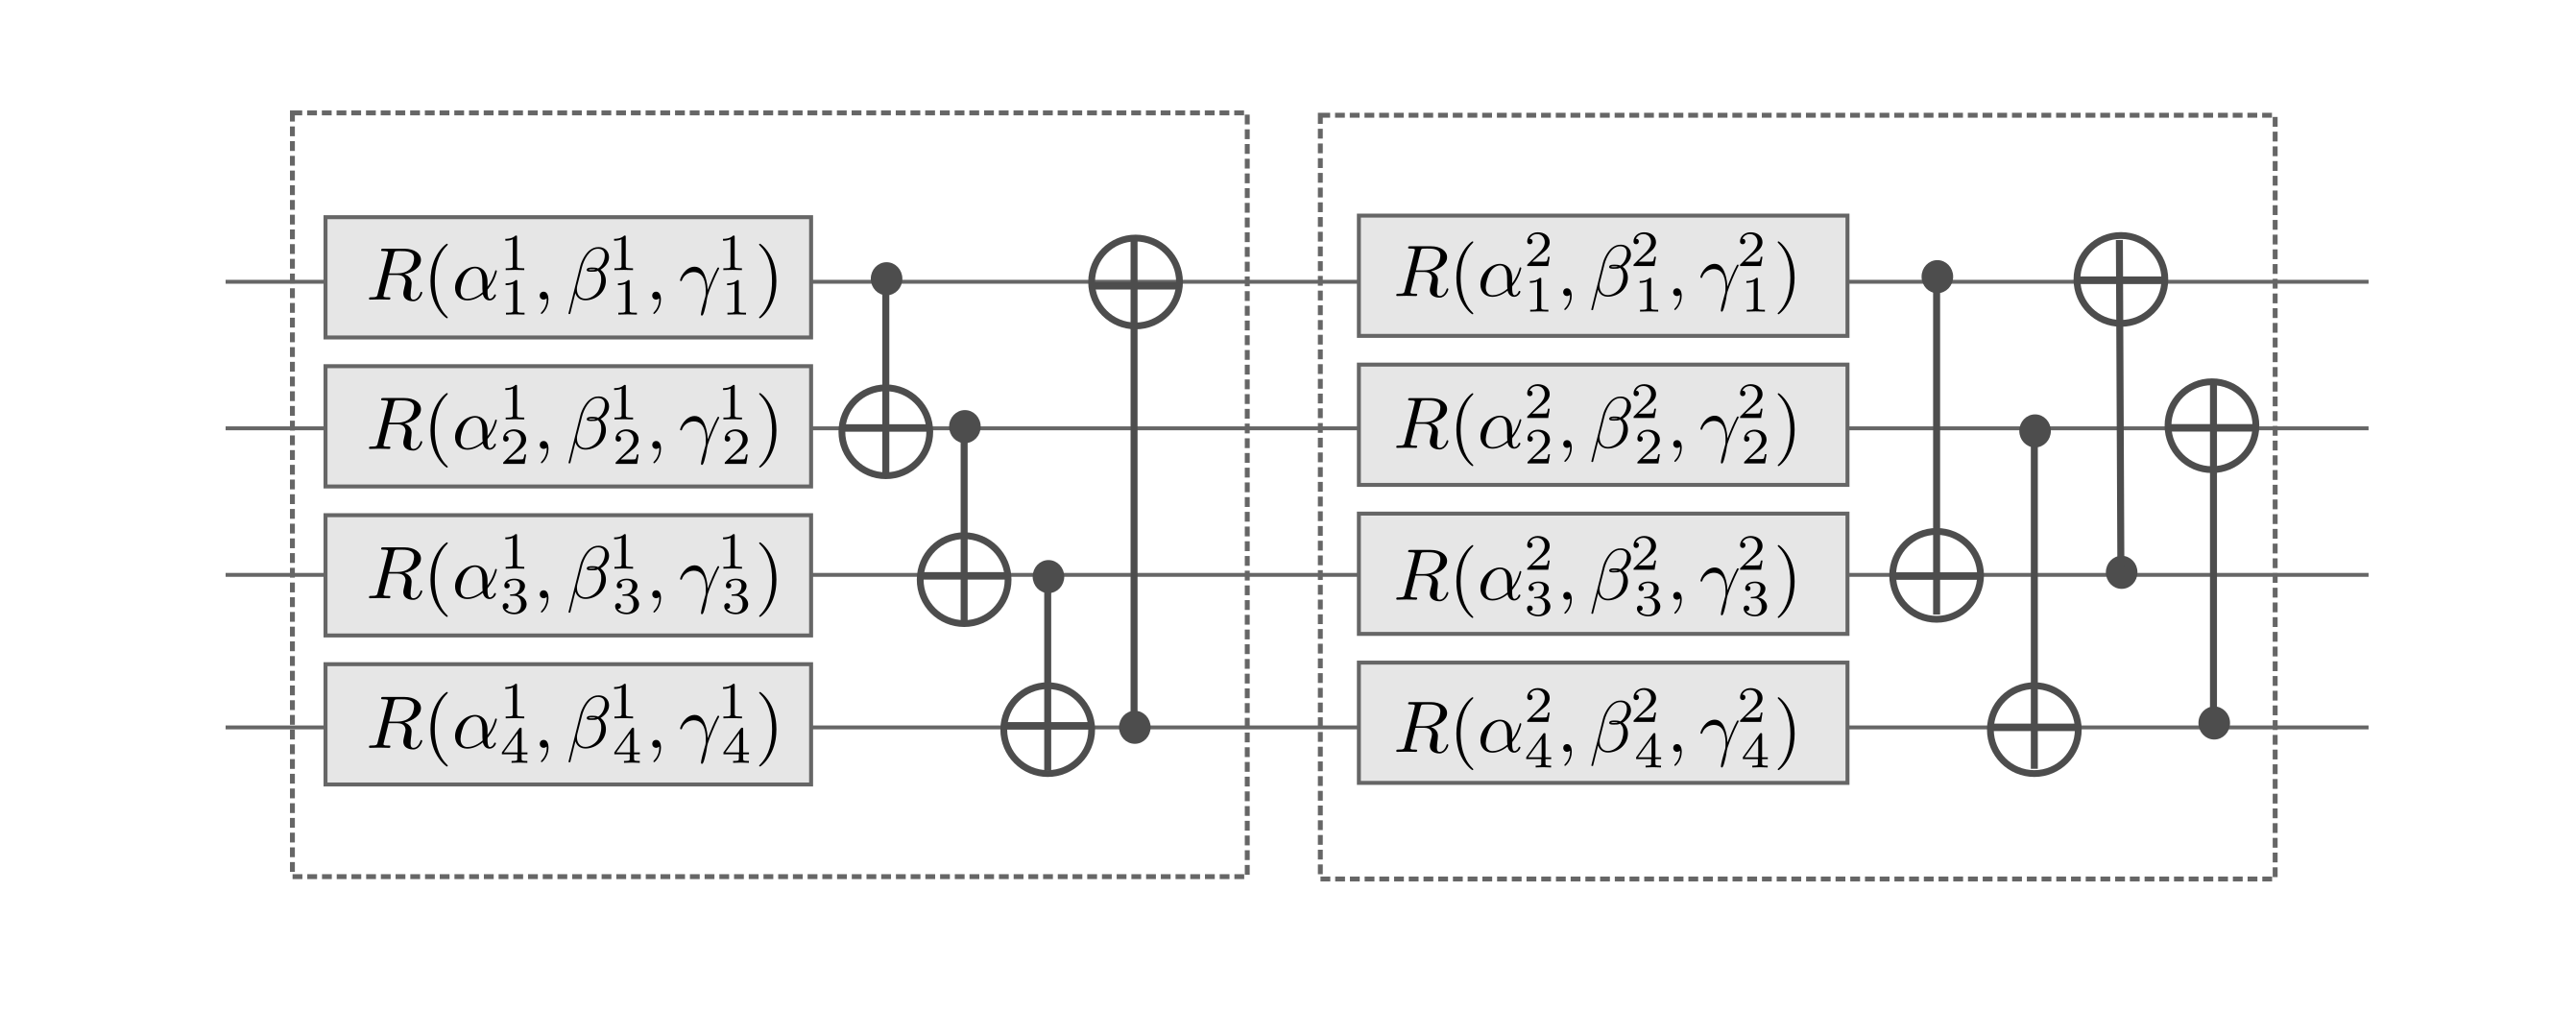
\includegraphics[width=8cm]{fig/layer_sec.png}};

		% Image 2: Bottom Right
		\node<2-> at ([shift={(-3cm,2cm)}]current page.south east)
		{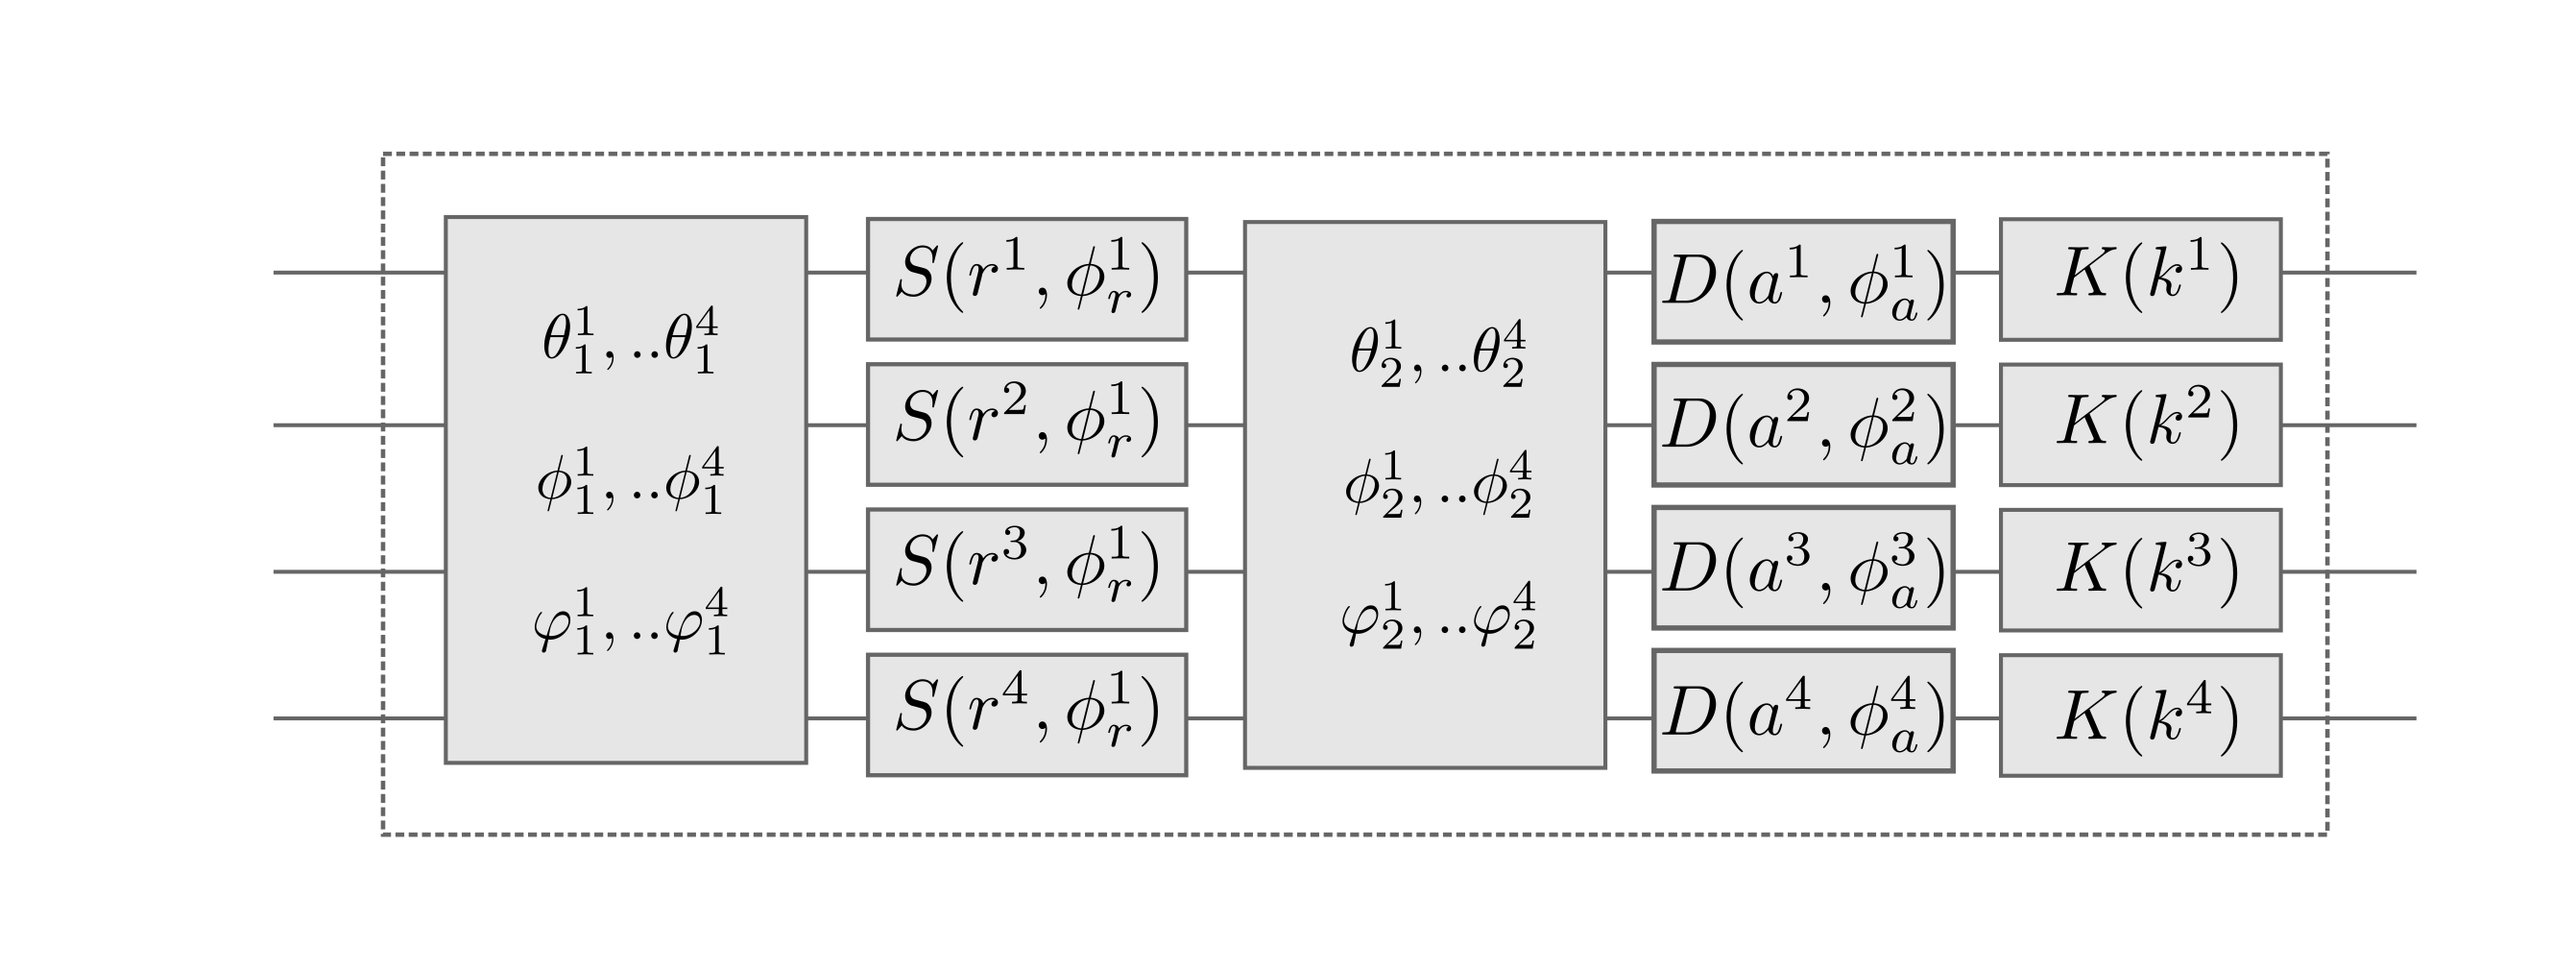
\includegraphics[width=8cm]{fig/layer_cvqnn.png}};

		% Image 3: Center-ish
		\node<1-> at ([shift={(1cm,0cm)}]current page.center)
		{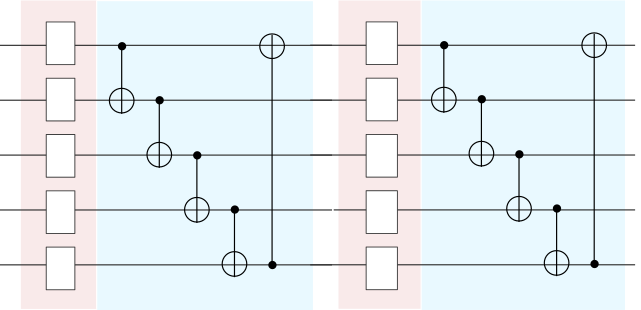
\includegraphics[width=8cm]{fig/basic_entangler.png}};

		% Image 4: Top Right
		\node<4-> at ([shift={(-4cm,-3cm)}]current page.north east)
		{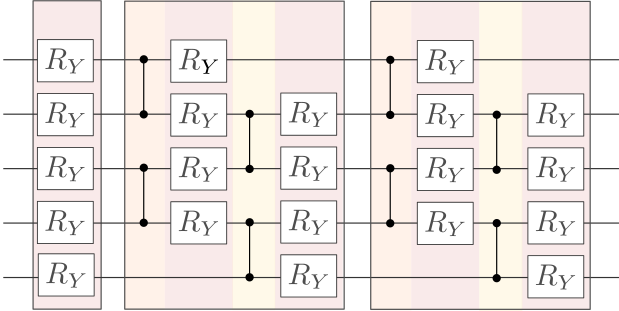
\includegraphics[width=8cm]{fig/simplified_two_design.png}};

		% Image 5: Bottom Left
		\node<5-> at ([shift={(4cm,2.5cm)}]current page.south west)
		{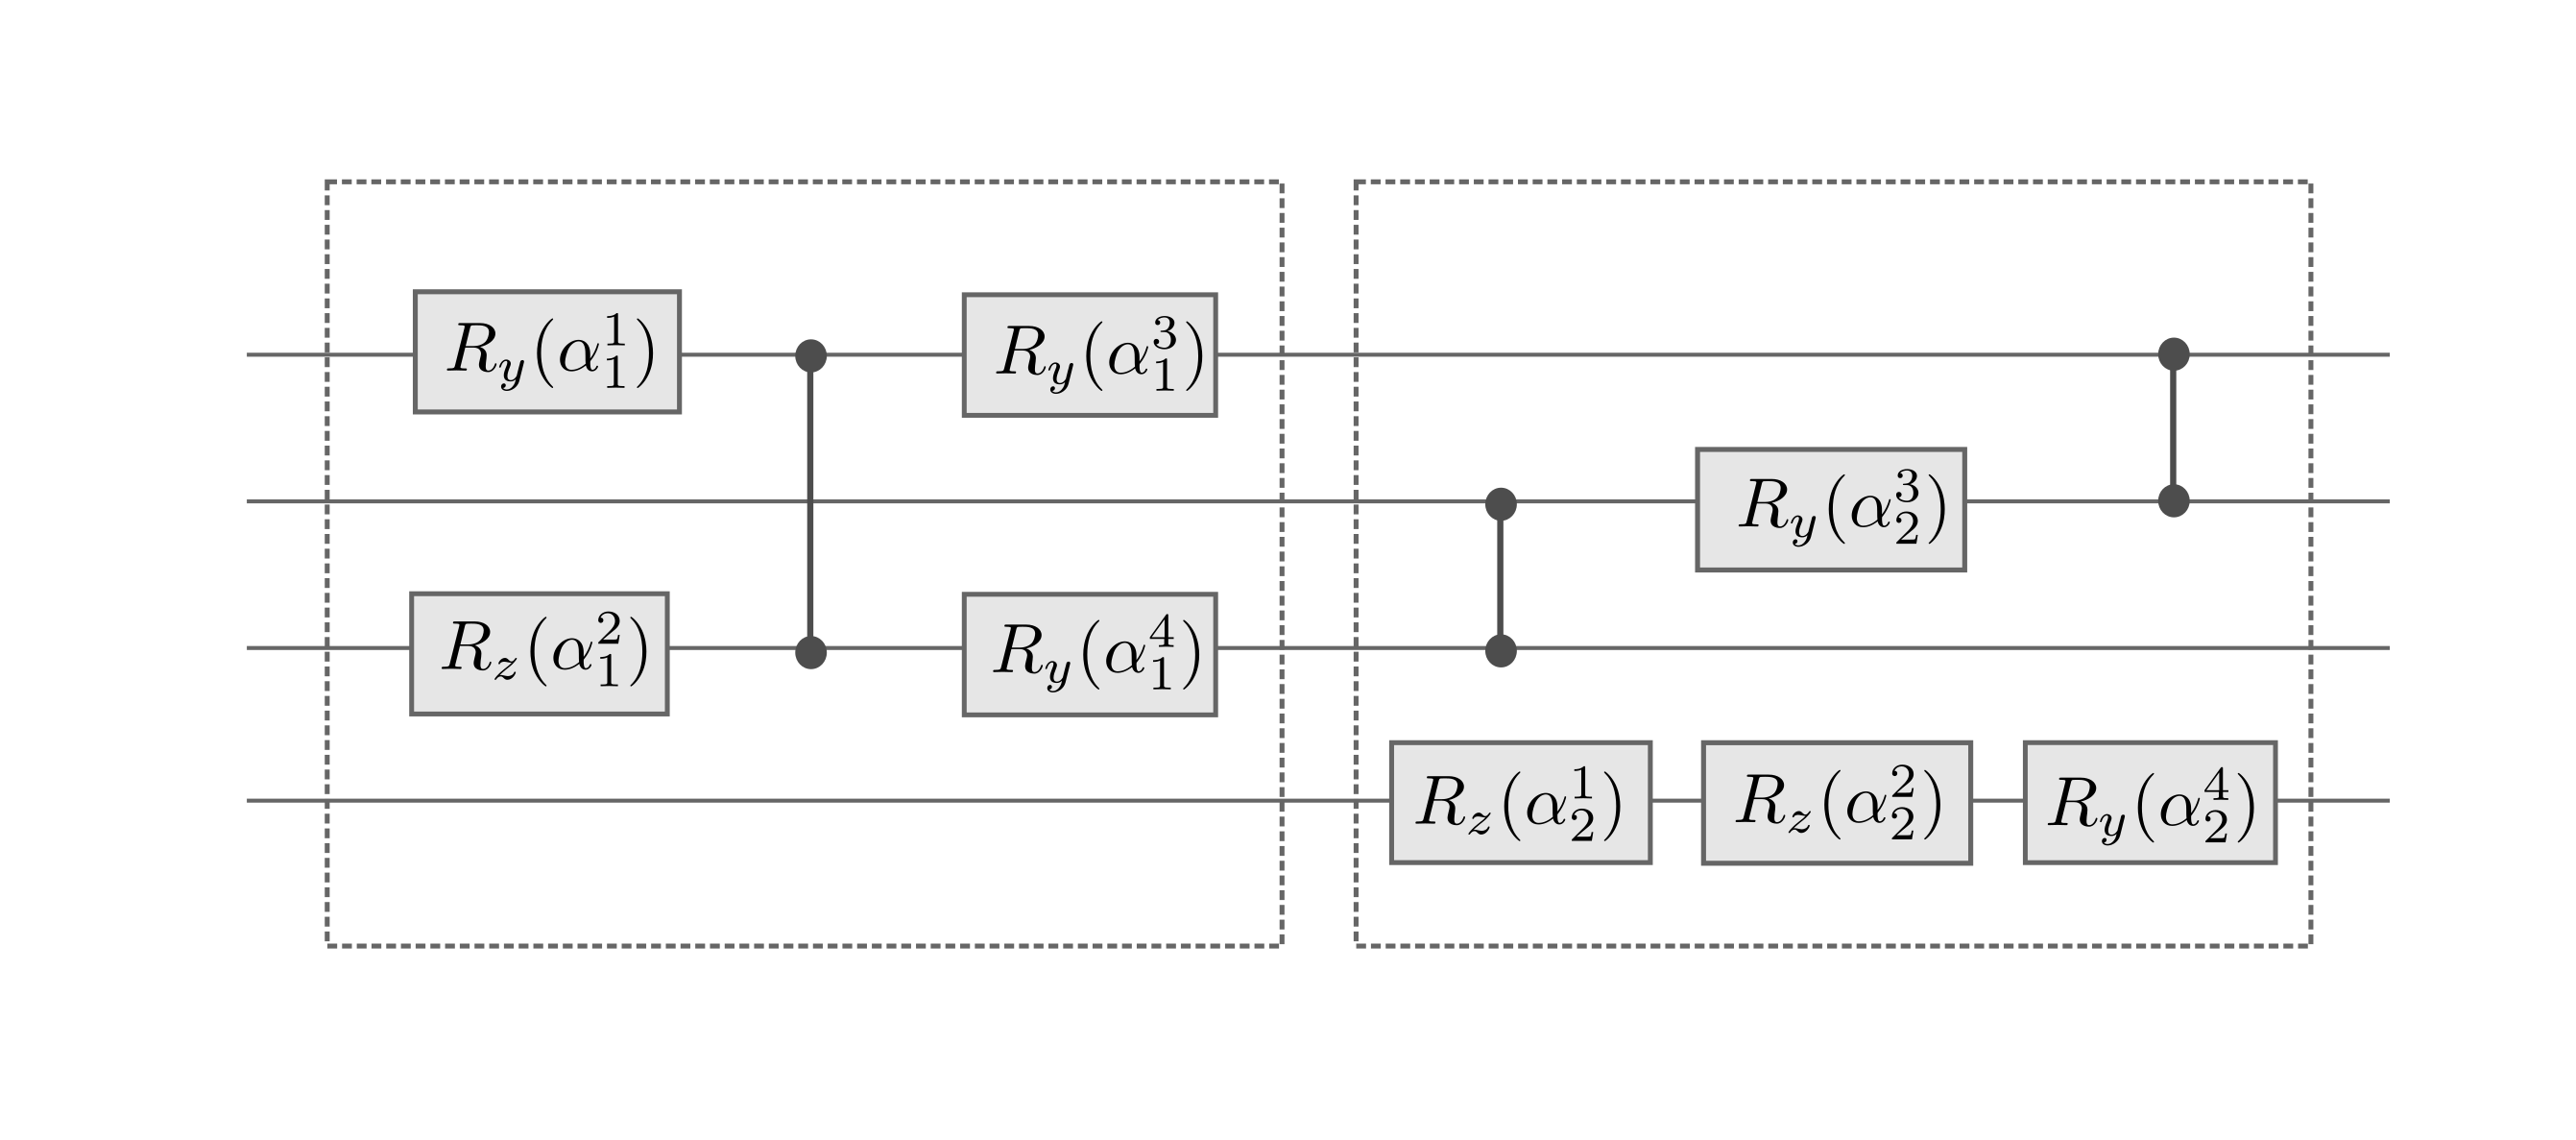
\includegraphics[width=8cm]{fig/layer_rnd.png}};
	\end{tikzpicture}
\end{frame}

\begin{frame}[fragile]{{Quantum Architecture Search (QAS)}}
	\begin{figure}
		\centering
		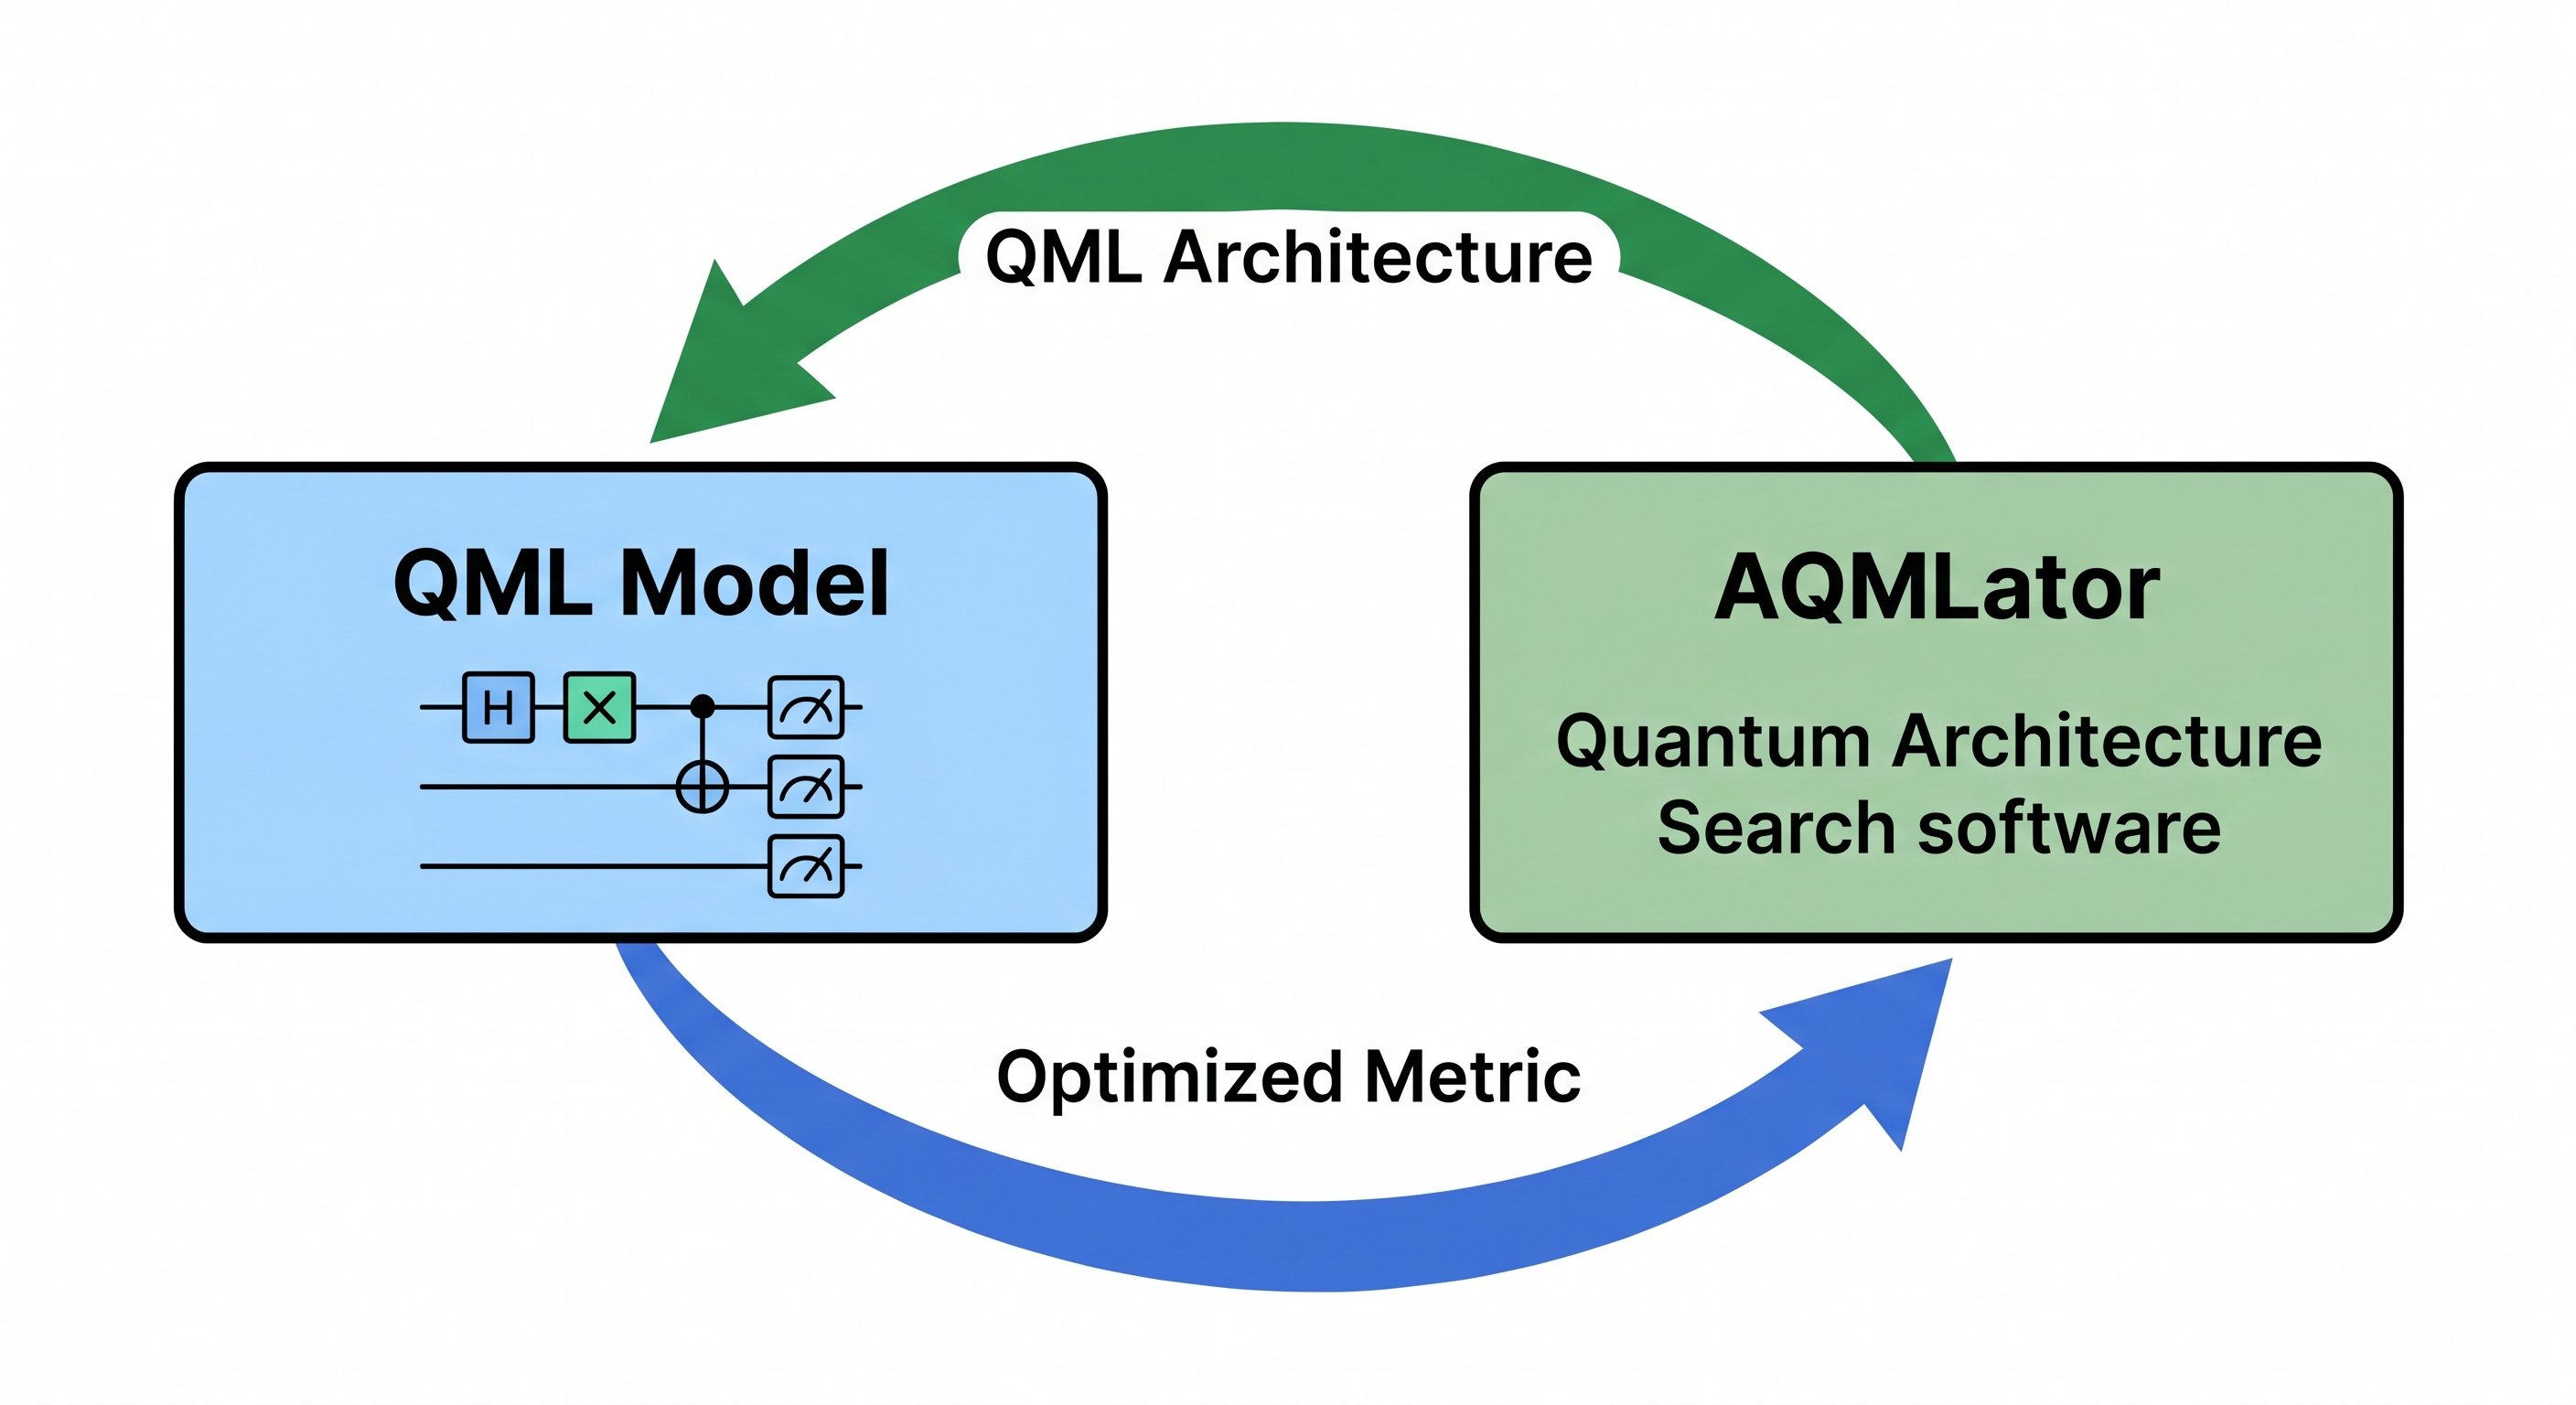
\includegraphics[width=1.0\textwidth]{fig/aqmlator_2.png}
		\label{fig:aqml}
	\end{figure}
\end{frame}

%%%%%%%%%%%%%%%%%%%%%%%%%%%%%%%%%%%%%%%%%%%%%%%%%%%%%%%%%%%%%%%%%%%%%%%%%%%%%%%%%%%%%%%%%%%%%%%%
% \part{Problem Formulation}

% \begin{frame}[fragile]{{Problem Formulation}}
% 	\alt<1>{
% 		\begin{alertblock}<1>{Problem I --- Data Fusion}
% 			Join information from multiple modalities (sources) to perform prediction
% 		\end{alertblock}
% 	}{
% 		\begin{block}<1->{Problem I --- Data Fusion}
% 			Join information from multiple modalities (sources) to perform prediction
% 		\end{block}
% 	}
% 	\alt<2>{
% 		\begin{alertblock}<2->{Problem II --- Change Detection}
% 			Given a pair of corresponding pictures, depicting the same region and taken at different times, find the regions that differ between the pictures
% 		\end{alertblock}
% 	}{
% 		\begin{block}<2->{Problem II --- Change Detection}
% 			Given a pair of corresponding pictures, depicting the same region and taken at different times, find the regions that differ between the pictures
% 		\end{block}
% 	}
% 	\alt<3>{
% 		\begin{alertblock}<3->{Problem III --- Quantum Architecture Search}
% 			Given the task and the search space, find within the search space a quantum circuits that best fits the task, according to predefined evaluation criteria.
% 		\end{alertblock}
% 	}{
% 		\begin{block}<3->{Problem III --- Quantum Architecture Search}
% 			Given the task and the search space, find within the search space a quantum circuits that best fits the task, according to predefined evaluation criteria.
% 		\end{block}
% 	}
% \end{frame}

%%%%%%%%%%%%%%%%%%%%%%%%%%%%%%%%%%%%%%%%%%%%%%%%%%%%%%%%%%%%%%%%%%%%%%%%%%%%%%%%%%%%%%%%%%%%%%%%

\begin{frame}[fragile]{{MNIST Multisource}}
	\begin{figure}
		\centering
		
\includegraphics[width=1.0\textwidth]{fig/preprocessing.pdf}
		\label{fig:mnist}
	\end{figure}
\end{frame}

\begin{frame}[fragile]{{Baseline Classical Neural Network}}
	\begin{figure}
		\centering
		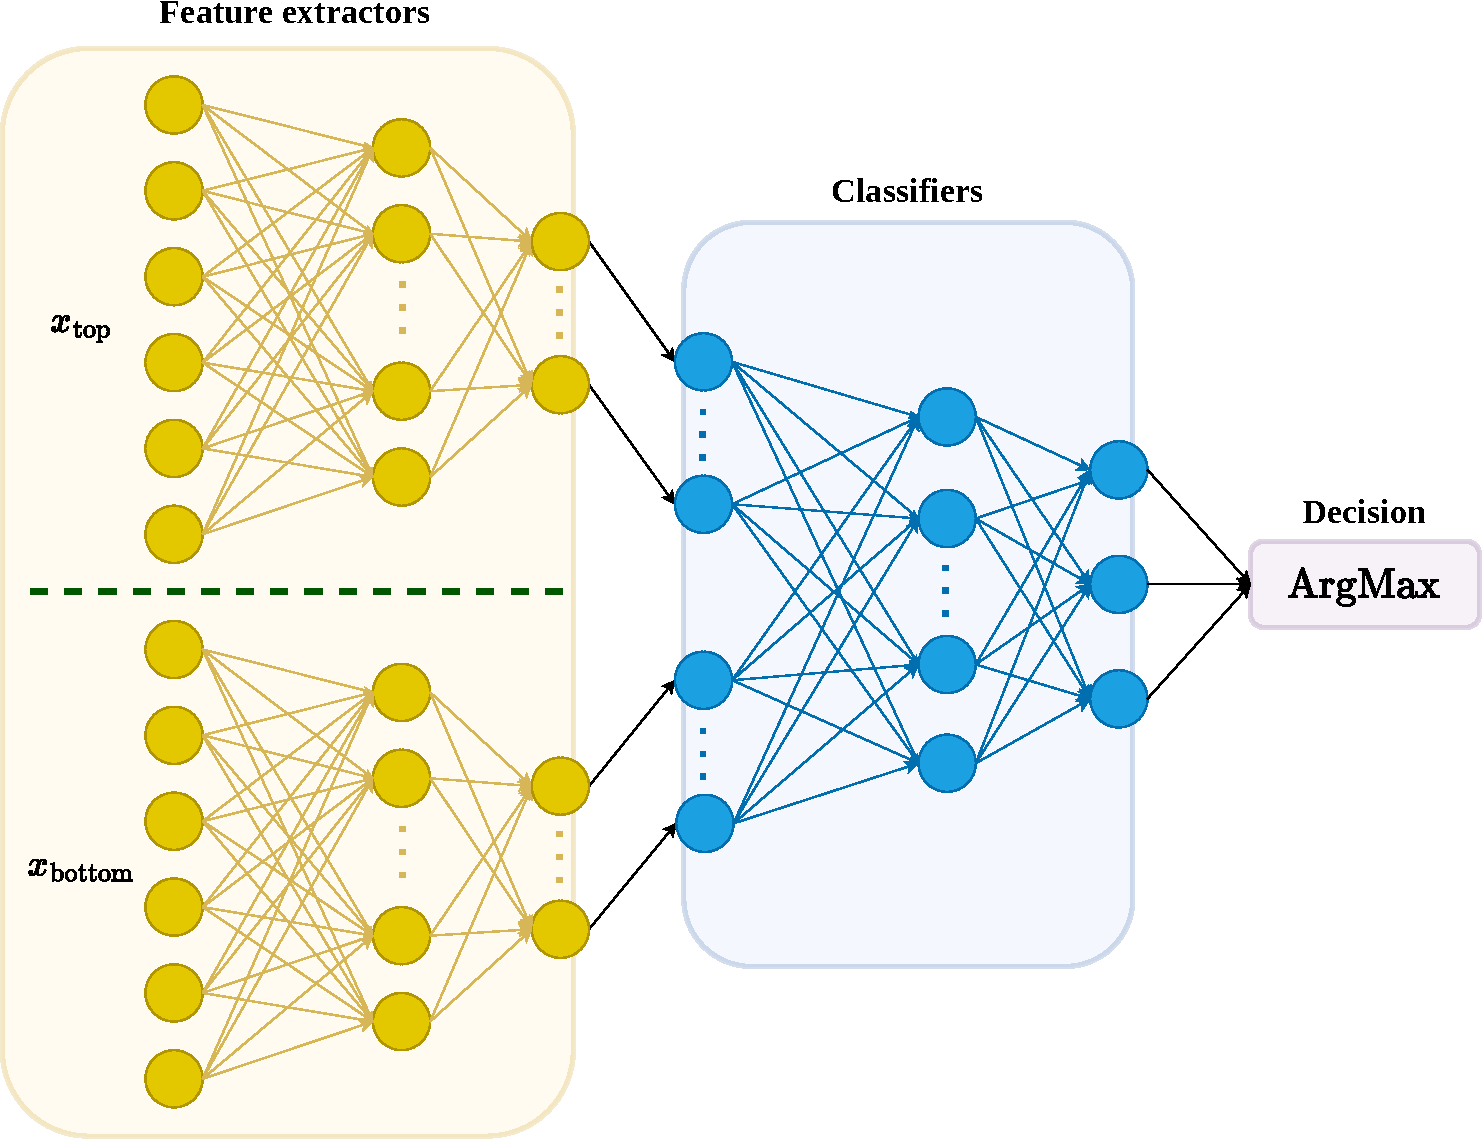
\includegraphics[width=0.8\textwidth]{fig/model_schema_mnist_classical.pdf}
		\label{fig:mnist_classical}
	\end{figure}
\end{frame}

\begin{frame}[fragile]{{Hybrid Quantum-Classical Neural Network}}
	\begin{figure}
		\centering
		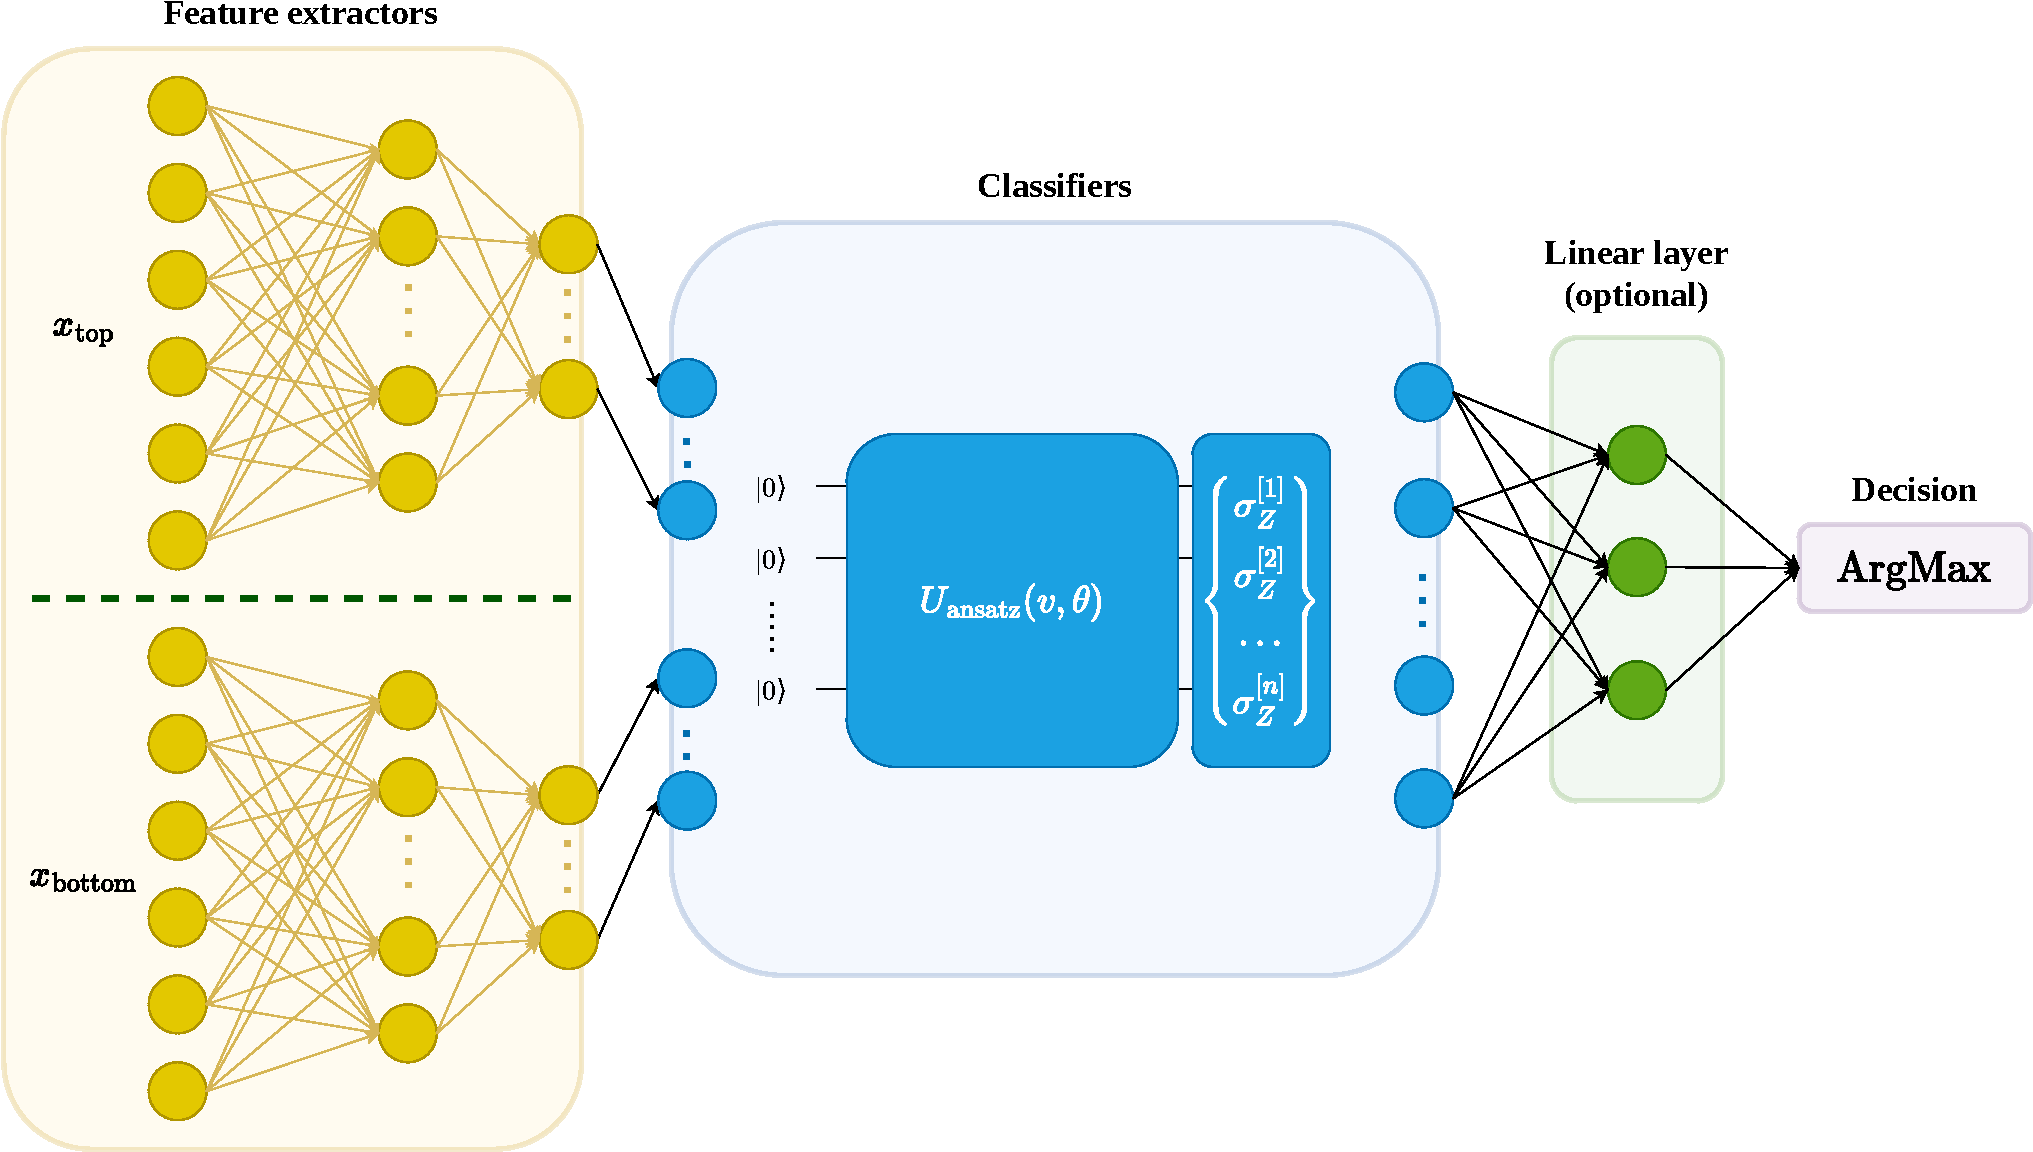
\includegraphics[width=1.0\textwidth]{fig/model_schema_mnist_quantum.pdf}
		\label{fig:mnist_quantum}
	\end{figure}
\end{frame}

\begin{frame}[fragile]{{MNIST}}
	\begin{table}[h]
		\centering
		\renewcommand{\arraystretch}{1.5}
		\setlength{\tabcolsep}{6pt}
		\caption{
			Accuracy metrics for our best classical, manual PQC and AQML-found PQC models.
			PQC$^{\mathrm{Solo}}_{\mathrm{AQML}}$ and PQC$^{\mathrm{Linear}}_{\mathrm{AQML}}$ denote PQC models without and with final classical linear layer respectively.
			We also provide trainable parameters number for each model.}
		\label{tab:mnist_results}
		\begin{tabular}{lccc}
			\hline
			\textbf{Model}                            & \textbf{Accuracy$\mathrm{\mathbf{_{best}}}$ (5-fold CV, mean ± SD)} & \textbf{\# Parameters} \\
			\hline
			{MLP}                                     & $\mathbf{0.960 \pm 0.001}$                                          & {75995}                \\
			{PQC$_{\mathrm{manual}}$}                 & $0.886 \pm 0.022$                                                   & \textbf{4632}          \\
			{PQC$^{\mathrm{Solo}}_{\mathrm{AQML}}$}   & $0.939 \pm 0.006$                                                   & {6274}                 \\
			{PQC$^{\mathrm{Linear}}_{\mathrm{AQML}}$} & $0.944 \pm 0.005$                                                   & {10899}                \\
			\hline
		\end{tabular}
	\end{table}
\end{frame}

%%%%%%%%%%%%%%%%%%%%%%%%%%%%%%%%%%%%%%%%%%%%%%%%%%%%%%%%%%%%%%%%%%%%%%%%%%%%%%%%%%%%%%%%%%%%%%%%
\begin{frame}[fragile]{{Change Detection}}
	\begin{block}{Change Detection}
		Given a pair of corresponding \textbf{multispectral} (13-band) images, depicting the same region and taken at different times, find the regions that differ between the pictures
	\end{block}
	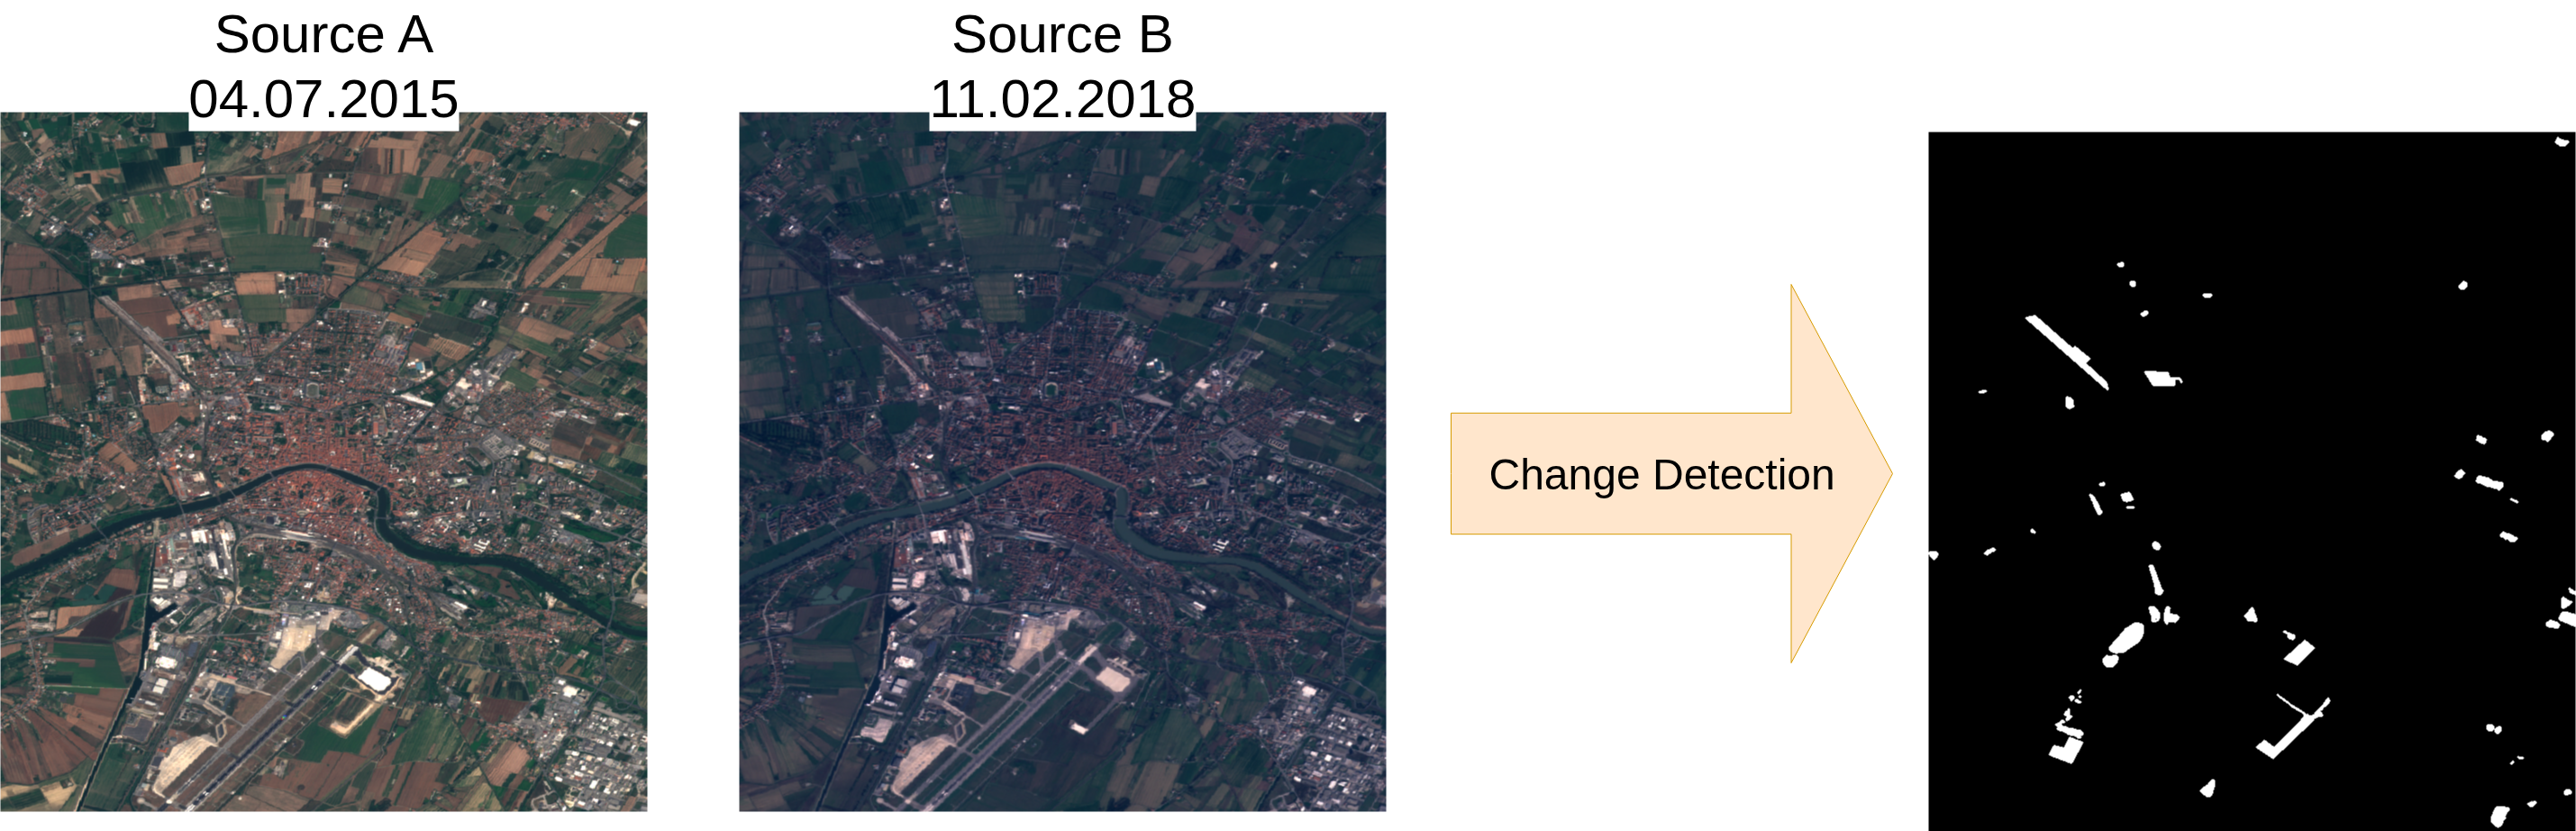
\includegraphics[width=1.0\textwidth]{fig/change_detection_horizontal.png}
\end{frame}

\begin{frame}[fragile]{{Baseline Classical Neural Network}}
	\begin{figure}
		\centering
		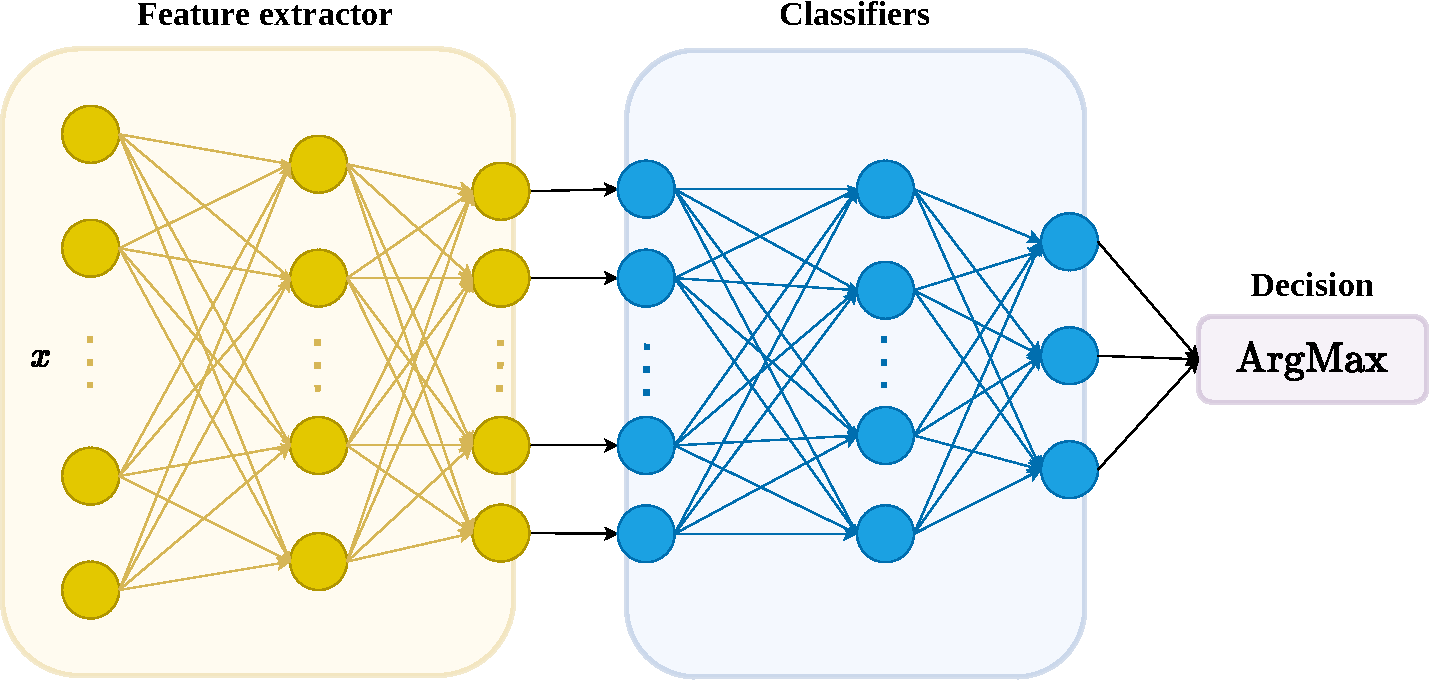
\includegraphics[width=0.8\textwidth]{fig/model_schema_onera_classical.pdf}
		\label{fig:onera_classical}
	\end{figure}
\end{frame}

\begin{frame}[fragile]{{Hybrid Quantum-Classical Neural Network}}
	\begin{figure}
		\centering
		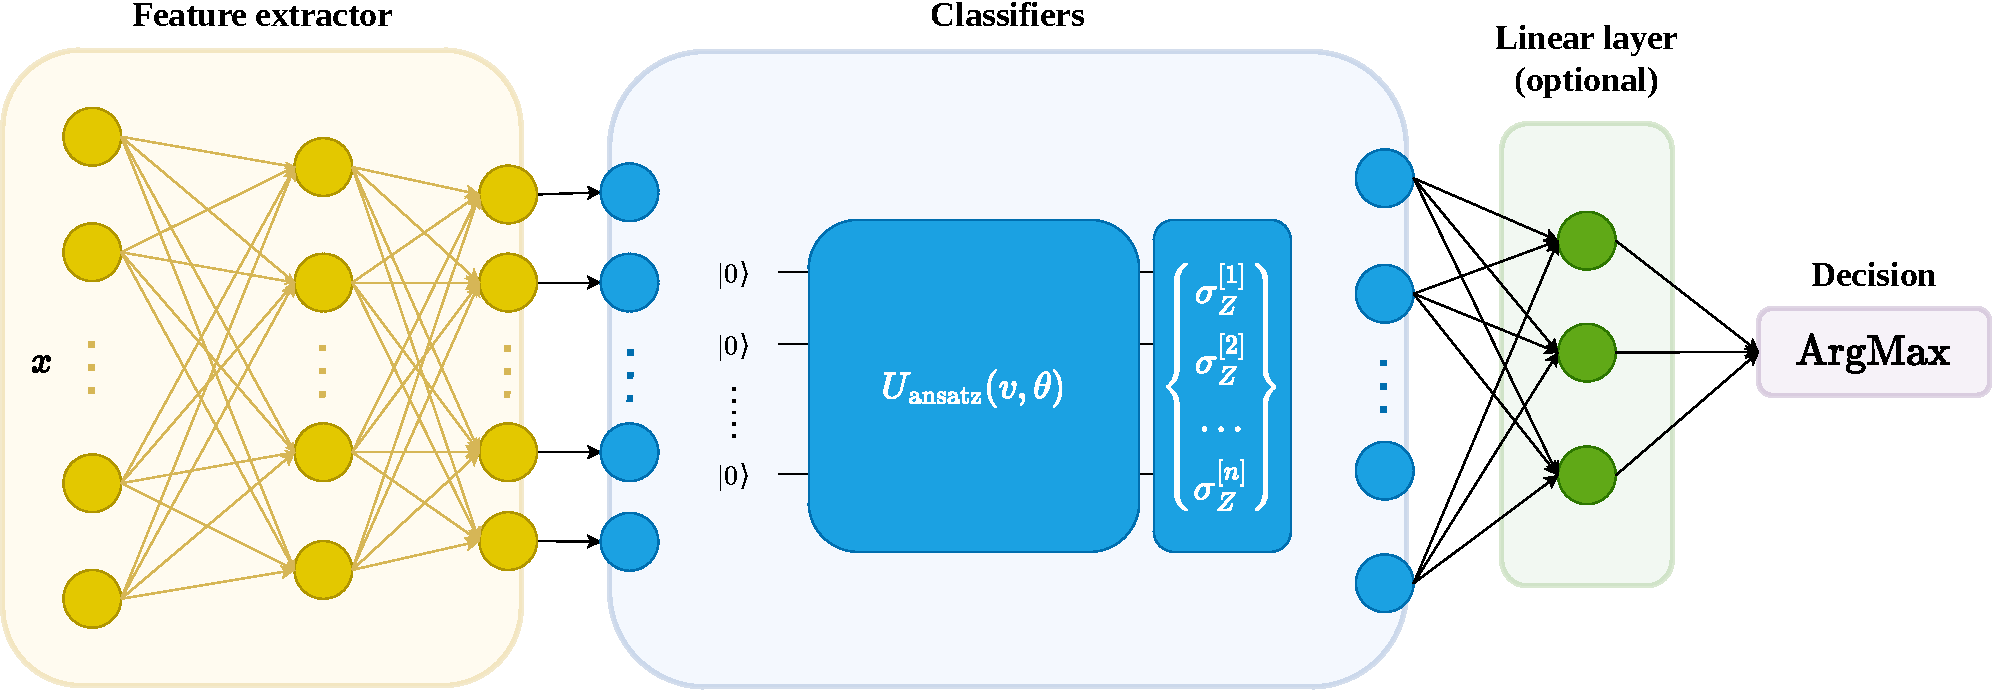
\includegraphics[width=1.0\textwidth]{fig/model_schema_onera_quantum.pdf}
		\label{fig:onera_quantum}
	\end{figure}
\end{frame}

\begin{frame}[fragile]{{OSCD — Onera Satellite Change Detection}}
	\begin{table}[h]
		\centering
		\renewcommand{\arraystretch}{1.5}
		\setlength{\tabcolsep}{6pt}
		\caption{
			Accuracy comparison for change detection on the OSCD dataset. PQC$_{\mathrm{Solo}}^{\mathrm{AQML}}$ is hybrid model without the linear layer,
			and  PQC$_{\mathrm{Linear}}^{\mathrm{AQML}}$ is with the linear layer.}
		\label{tab:onera_results}
		\begin{tabular}{lcccc}
			\hline
			\textbf{Model}                          & $\mathbf{acc_{best}}$ & $\mathbf{acc_{avg}}$ & $\mathbf{acc_{min}}$ & \textbf{\# Parameters} \\
			\hline
			MLP (6 layers)                          & \textbf{0.752}        & 0.728                & --                   & 384                    \\
			MLP (1 layer)                           & 0.738                 & \textbf{0.731}       & --                   & 64                     \\
			PQC$_{\mathrm{Solo}}^{\mathrm{AQML}}$   & 0.738                 & 0.676                & 0.505                & \textbf{8--72}         \\
			PQC$_{\mathrm{Linear}}^{\mathrm{AQML}}$ & 0.743                 & 0.730                & \textbf{0.710}       & 8--135                 \\
			\hline
		\end{tabular}
	\end{table}
\end{frame}

%%%%%%%%%%%%%%%%%%%%%%%%%%%%%%%%%%%%%%%%%%%%%%%%%%%%%%%%%%%%%%%%%%%%%%%%%%%%%%%%%%%%%%%%%%%%%%%%
% \part{Conclusions}
\begin{frame}[fragile]{{Conclusions}}
	\begin{enumerate}[<+-|alert@+>]
		\item \textbf{Automated Optimization:} Even basic Automated Quantum Machine Learning (AQML) consistently outperforms manually selected quantum architectures.
		\item \textbf{Performance Gap:} While quantum models did not surpass the best classical benchmarks, they achieved comparable accuracy levels.
		\item \textbf{Parameter Efficiency:} Quantum models reached competitive performance using significantly fewer trainable parameters than their classical counterparts.
	\end{enumerate}
	\onslide
\end{frame}


\begin{frame}[fragile]{{Ending}}
	\centering{\Large Thank you for attention}

\end{frame}


%%%%%%%%%%%%%%%%%%%%%%%%%%%%%%%%%%%%%%%%%%%%%%%%%%%%%%%%%%%%%%%%%%%%%%%%%%%%%%%%%%%%%%%%%%%%%%%%%%%%%%%%%%%%%%%%%%%%%%%%%%%%%%%%%%%%%%%%%%%%%%%%%%%%%%%%%%%%%%%%%%%%%%%%%%%%%%%%%%%%%%%%%%%%%%%%
%%%%%%%%%%%%%%%%%%%%%%%%%%%%%%%%%%%%%%%%%%%%%%%%%%%%%%%%%%%%%%%%%%%%%%%%%%%%%%%%%%%%%%%%%%%%%%%%%%%%%%%%%%%%%%%%%%%%%%%%%%%%%%%%%%%%%%%%%%%%%%%%%%%%%%%%%%%%%%%%%%%%%%%%%%%%%%%%%%%%%%%%%%%%%%%%
%%%%%%%%%%%%%%%%%%%%%%%%%%%%%%%%%%%%%%%%%%%%%%%%%%%%%%%%%%%%%%%%%%%%%%%%%%%%%%%%%%%%%%%%%%%%%%%%%%%%%%%%%%%%%%%%%%%%%%%%%%%%%%%%%%%%%%%%%%%%%%%%%%%%%%%%%%%%%%%%%%%%%%%%%%%%%%%%%%%%%%%%%%%%%%%%

\end{document}
